% !TeX root = main.tex
% !TeX spellcheck = en_US

\documentclass[aspectratio=169,9pt]{beamer}

\usepackage{royslides}
\usepackage{graphicx}     % More options for \includegraphics
\graphicspath{{figures/}} % Setting the graphicspath




\title{Quantum advantage using high-dimensional twisted photons as quantum finite automata}
\date{Milan University, 2022}
\author{Roy Stegeman}
\institute{University of Milan and INFN Milan}



% Overview
  % Finite Automata
  % Structured photon
% Finite Automata
% Structured photon
% Photonic Qubits
% 4-Qubit Photonic QFA
% Experiment
% Measurement
% Results 
  % 1-Qubit
  % Multi-Qubit(more efficient than single qubit, lower accepting probability)
% Summary
  % Photonic realization of QFA
  % Strucutred photons as multi-qubit states
  % Demonstrates state efficiency with 2-qubit QFA compared to classical FA (4 states vs 5)



\begin{document}
% TITLEPAGE ====================================================================
{
\setbeamertemplate{headline}{} % remove headline from titlepage
\begin{frame}
  \titlepage


  Based on arXiv:2202.04915

\end{frame}
}


% INTRO ========================================================================

\begin{frame}[t]{Content}
  \begin{itemize}
    \item This paper: detecting prime numbers with QFAs using structured photons
    \item What is QFA?
    \item What are twisted photons?
    \item Experimental setup
    \item Results
  \end{itemize}
\end{frame}


% QUANTUM FINITE AUTOMATA ======================================================
\section{Quantum Finite Automata}
\begin{frame}[t]{Finite State Automaton}
  \begin{itemize}
    \item abstract machine (very simple computational model) that can be in exactly one of a finite number of states at a given time
    \item State can change from one to another as response to inputs
    \item FSA is defined by initial state, list of states and ipnuts that trigger each transition (think elevator or combination lock)
    \item Memory of a FSA is represented by the finite number of states in which a FSA can be
    \item FSA can be deterministic (will explain first for simplicity) or probabilistic (a QFA is probabilistic)
  \end{itemize}
\end{frame}


\begin{frame}[t]{Deterministic Finite Automata}
  \begin{itemize}
    \item $MOD_n=\{a^j|j \mod n \equiv 0 \}$ for $n>1$
    \item decision problem: is the lengtho f an input string a multiple of $n$ or not?
    \item (a) simple example of graph representation
    \item (b) representation of our $MOD_n$ problem (only accepting state is $s_0$):\\
    for each symbol $a$, the DFA performs a transition between the states\\
    so after if the length is a multiple of $n$, the system transitions back to its initial (and only accepting) state. Hence $MOD_n$ langauge.
    \item \textbf{There is no DFA with less than $n$ states for $MOD_n$}

    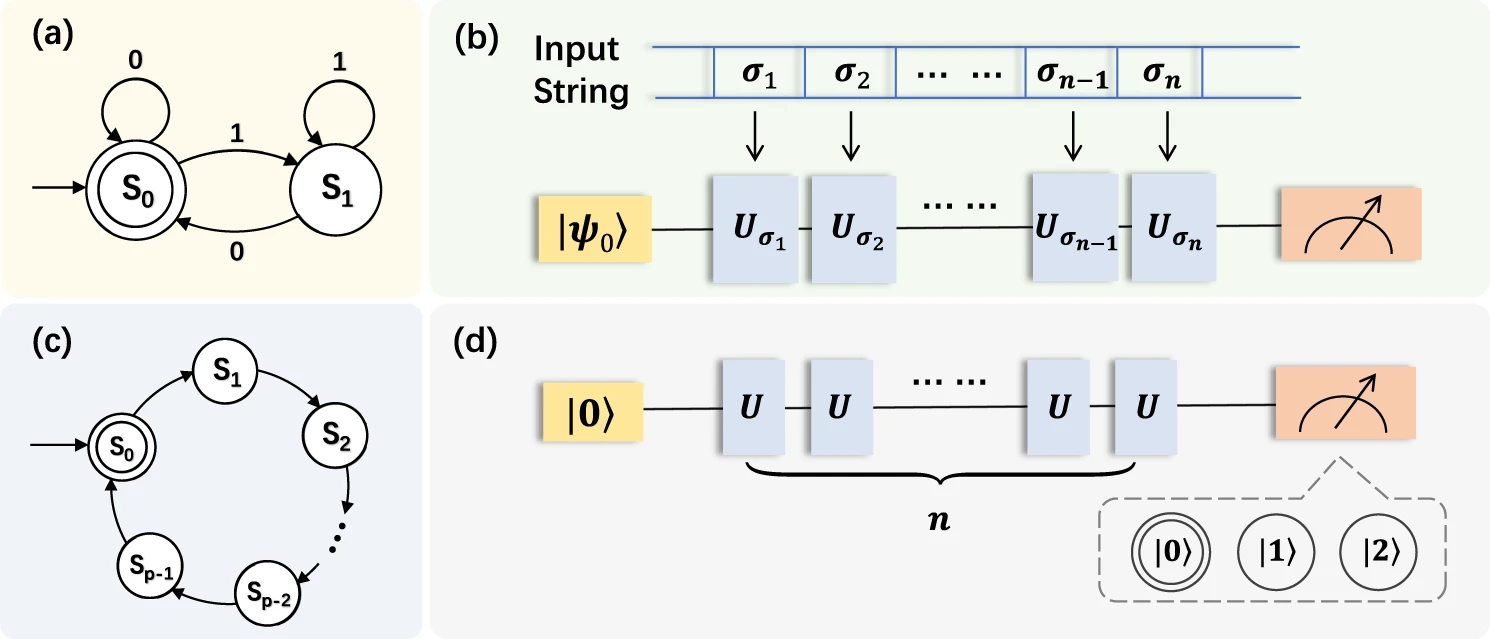
\includegraphics[width=0.4\textwidth]{DFA.png}\\
    Source: https://www.nature.com/articles/s41534-019-0163-x
  \end{itemize}
\end{frame}


\begin{frame}[t]{Probabilitic Finite Automata}
  \begin{itemize}
    \item can make more than one tranisition with probabilities that sum to one
    \item The input $x=x[1] x[2] \cdots x[l]$ can be traced linearly
    \item at any step the PDFA is in a probability distribution of its states represented by $v=\left(\begin{array}{llll}p_{1} & p_{2} & \cdots & p_{m}\end{array}\right)^{T}$
    \item transformation: $v_{f}=A_{\$} A_{x[l]} A_{x[l-1]} \cdots A_{x[1]} A_{\mathbb{C}} v_{0}$
    \item probablity of accepting $x$ is the sum of probablities corresponding to the accepting states in $v_f$
  \end{itemize}
\end{frame}



\begin{frame}[t]{Quantum Finite Automata}
  \begin{itemize}
    \item Quantum counter part of PFA
    \item QFA with $m$ basis states: $N=\left\{\left|q_{1}\right\rangle, \ldots,\left|q_{m}\right\rangle\right\}$
    \item $\left|v_{f}\right\rangle=U_{\$} U_{x[l]} U_{x[l-1]} \cdots U_{x[1]} U_{\mathbb{C}}\left|v_{0}\right\rangle$
    \item $\sum_{q_{j} \in N_{a}}\left|\left\langle q_{j} \mid v_{f}\right\rangle\right|^{2}$, $N_a$ are the accepting states
    \item \textbf{Very similar to PFA but exponentially smaller than any classical (even randomized) FA (Ambainis and Freivalds, 1998)}
  \end{itemize}
\end{frame}


\begin{frame}[t]{2-state QFA}
  \begin{itemize}
    \item Two basis states: $|0\rangle,|1\rangle$ ($|0\rangle$ is the accepting state)
    \item Identity applied when reading $\$,\mathbb{C}$ 
    \item Input $x=a^n$, each a rotates by $\theta=2\pi/p$, thus reading of $a$
    leads to $U_{a}=\left(\begin{array}{rr}\cos \theta & -\sin \theta \\ \sin \theta & \cos \theta\end{array}\right)$
    \item thus the final state is $\left|v_{f}\right\rangle=\left(\begin{array}{c}\cos n \theta \\ \sin n \theta\end{array}\right)$
    \item Input accpted with $\cos^2(n\theta)$
    \item False acceptance rate
    \item 2d-state QFA reduced false acceptance rate of 2-state QFA
    \item Different acceptance rate for differnet $k$ run in parallel
    \item Eq. (14)
  \end{itemize}
\end{frame}



% EXPERIMENTAL SETUP ===========================================================
\section{Experimental Setup}

\begin{frame}[t]{QFA using photon OAM}
  \begin{itemize}
    \item QFA alorithm for MODp is one of the first quantum alogirhtms with exponental advantage over classical methods
    \item Performing the calculation on a quantum computer bacame random iddediately after reading a few symbols due to relateveily large noise in the copmutation process.
    \vspace*{1em}
    \item LG mode as lab realization of high-dimensional quantum states
    \item all modes are orthoganol
    \item the modes have high-diemnsional states (infintely many)
    \item used to encode single photons with quantum states
  \end{itemize}
  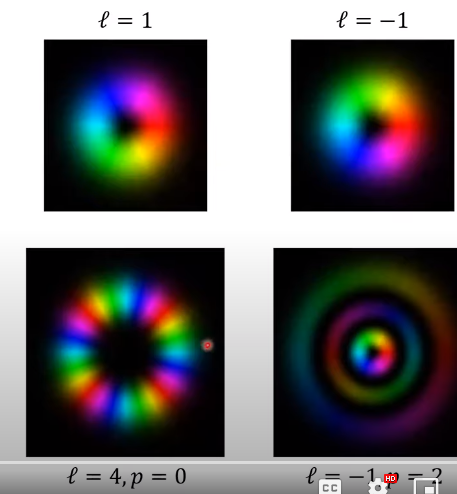
\includegraphics[width=0.2\textwidth]{LG_modes_structured_photons.png}
\end{frame}


\begin{frame}[t]{Photonic Qubit}
  \begin{itemize}
    \item physical realizaiton of a qubit
    \item $|\psi\rangle=\cos(\theta/2)|L_1\rangle + e^{i\phi}\sin(\theta/2)|L_{-1}\rangle$
  \end{itemize}
  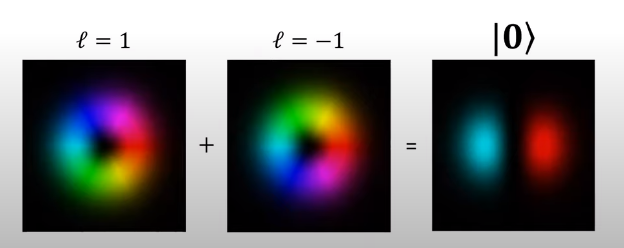
\includegraphics[width=0.2\textwidth]{photonic_superposition_qubit.png}
  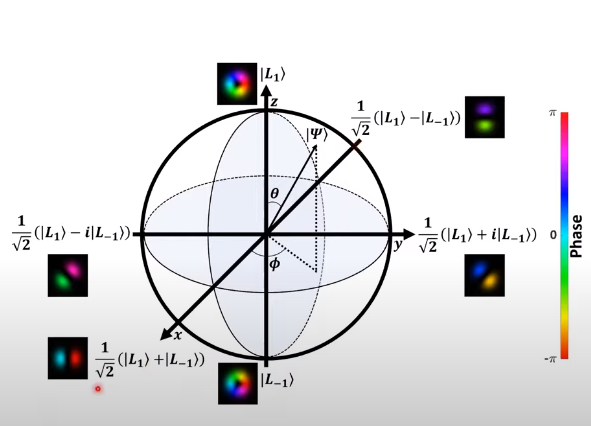
\includegraphics[width=0.2\textwidth]{photonic_bloch_sphere.png}
\end{frame}

\begin{frame}[t]{Photonic Qubit}
  Superposition correpond to the multiple 2-steate QFA of the theory part(?)
  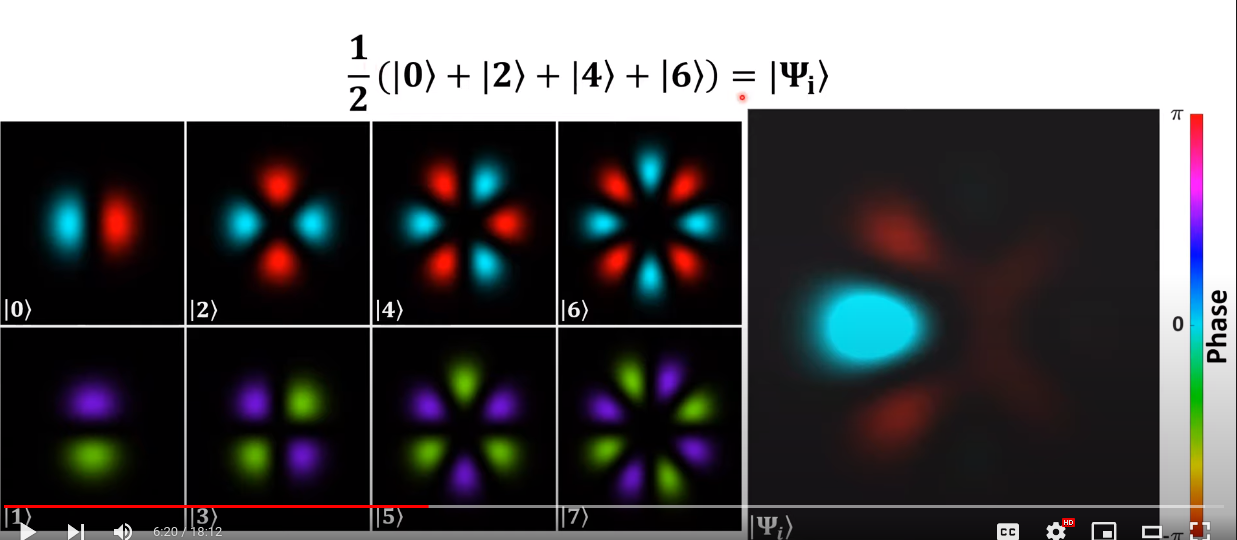
\includegraphics[width=0.5\textwidth]{4photon_qubit_superposition.png}
\end{frame}


\begin{frame}[t]{Experimental setup}
  \begin{itemize}
    \item Heralded single photons pass through first SLM
    \item Spatial light modulation
  \end{itemize}
  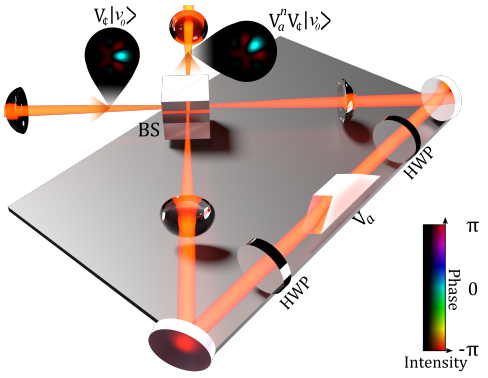
\includegraphics[width=0.3\textwidth]{experimental_setup.png}\\
  Loop that performs the unitary operation on the input state
  Remember eq(14)
\end{frame}


\begin{frame}[t]{Measurement}
  \begin{itemize}
    \item principle used for prime number search
    \item example: prime number 5
  \end{itemize}
  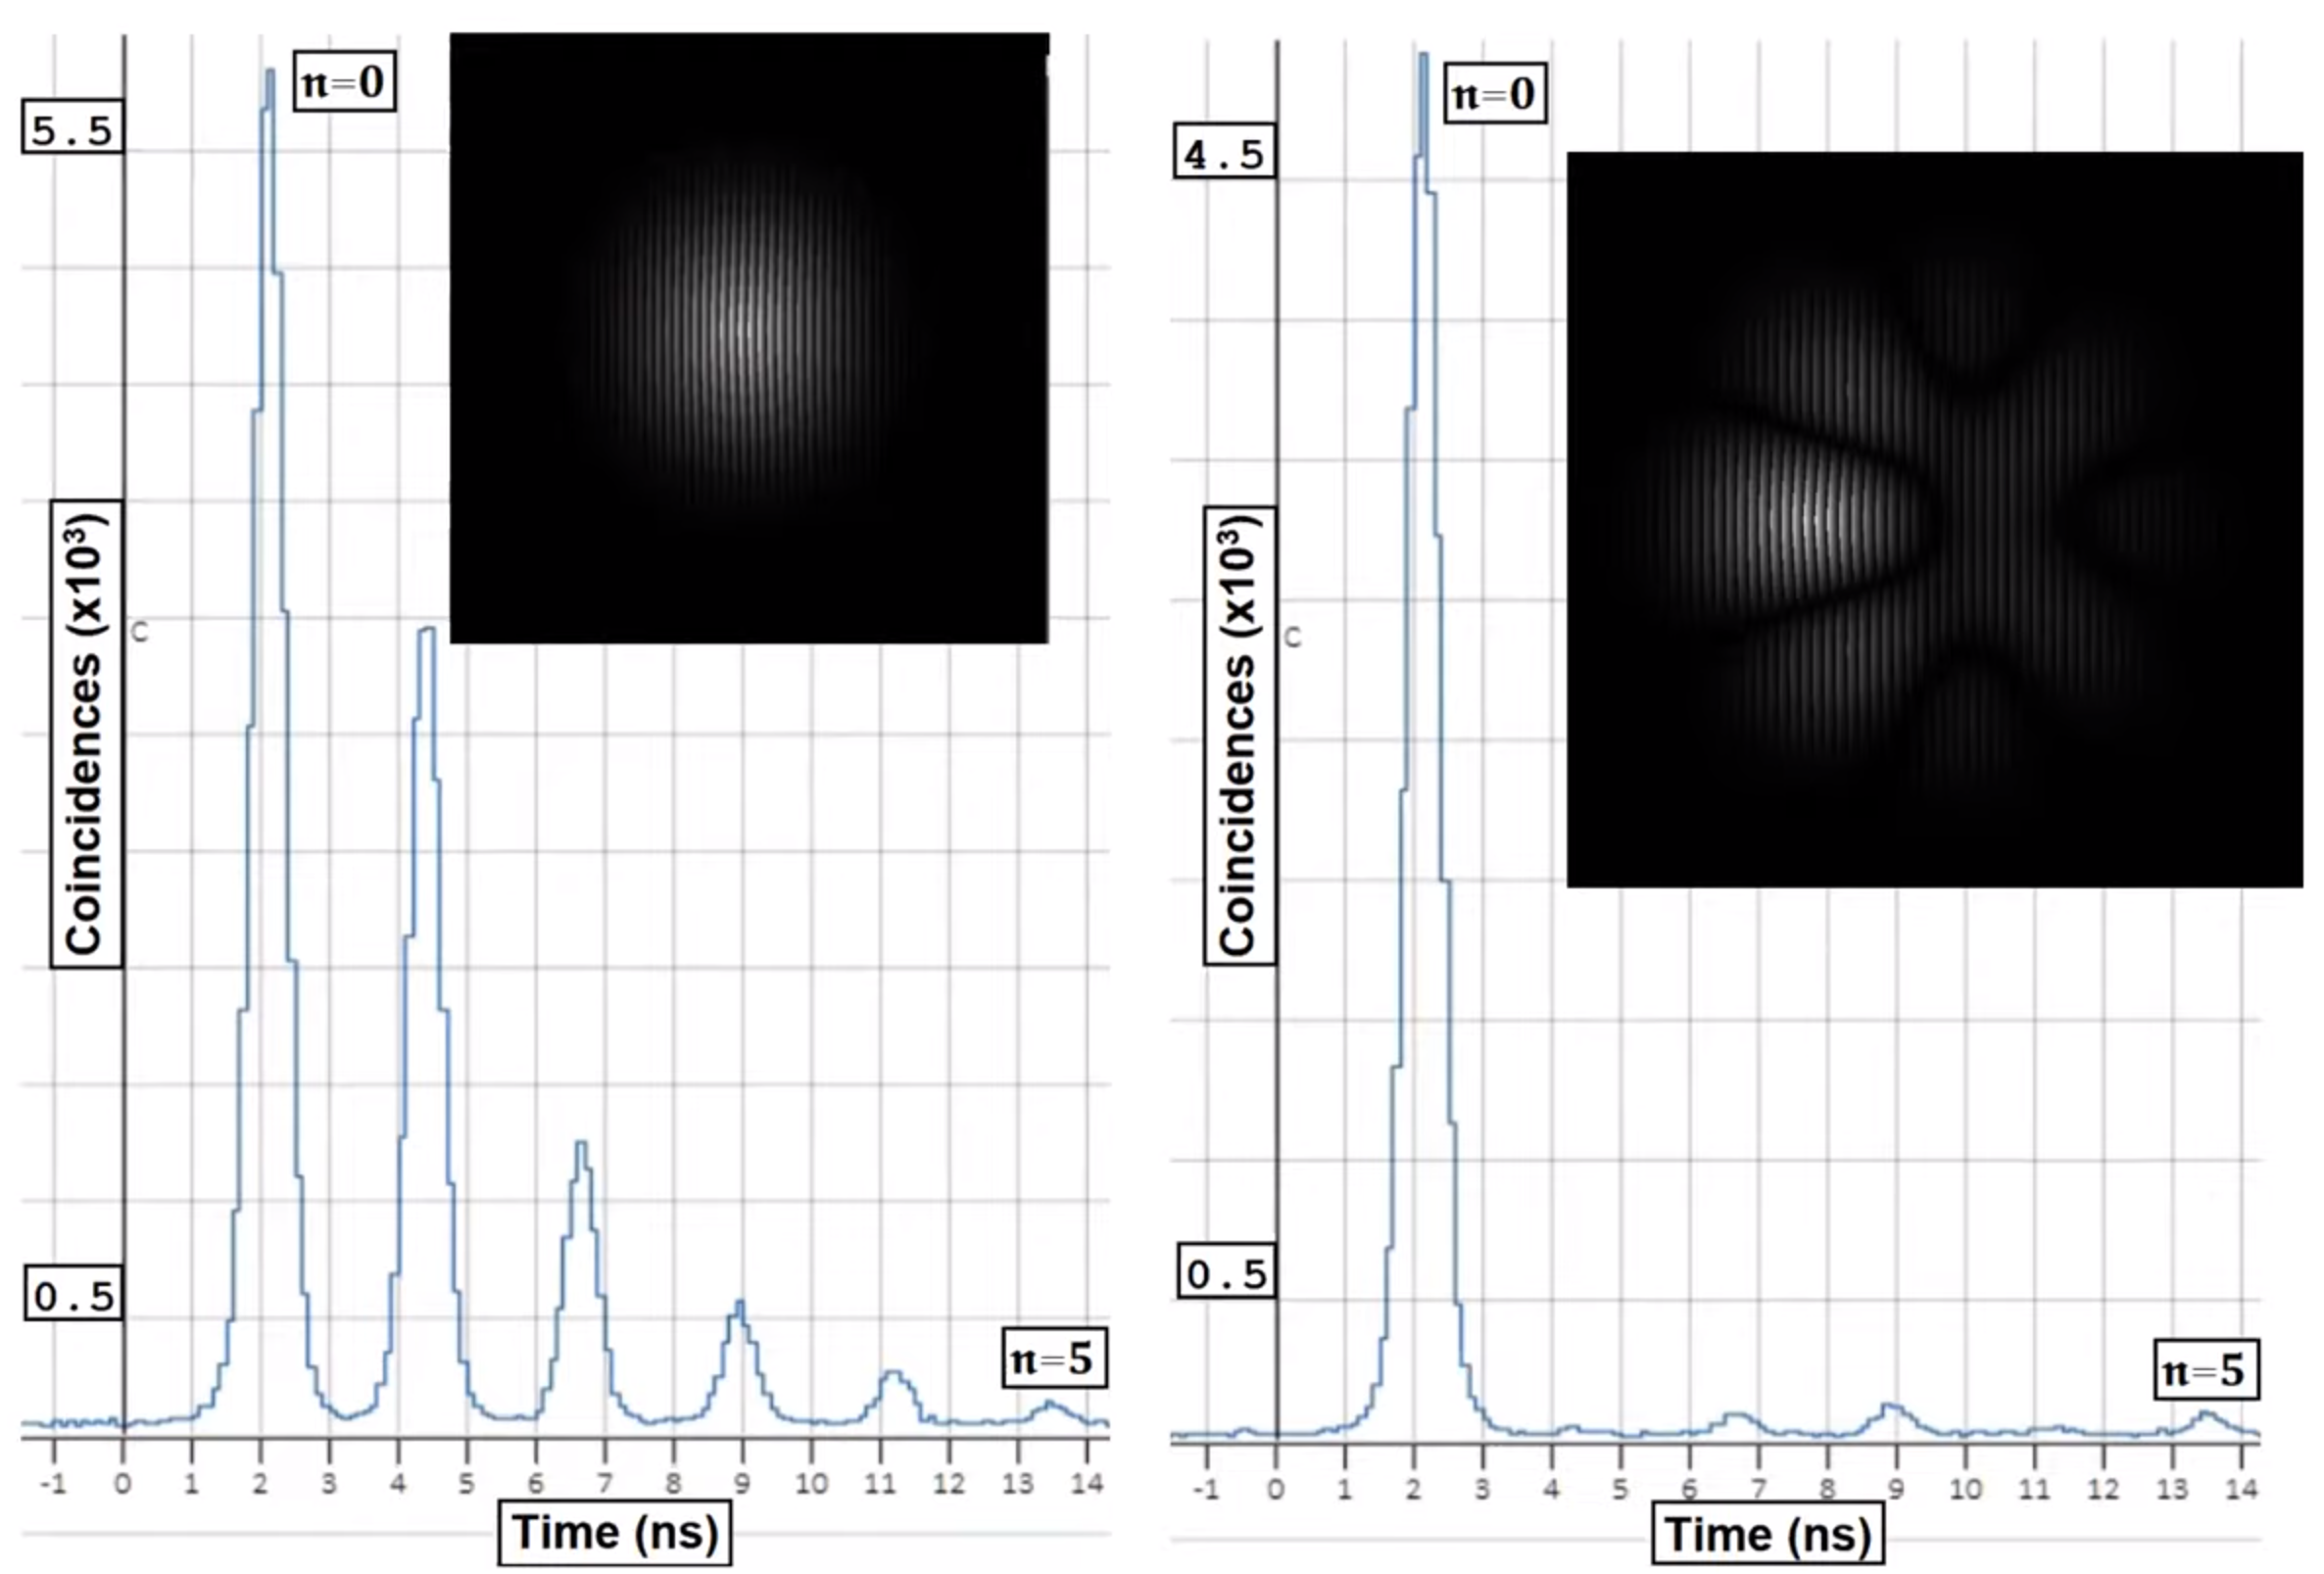
\includegraphics[width=0.3\textwidth]{example_measurement.png}
\end{frame}


% RESULTS ======================================================================
\section{Results}
\begin{frame}[t]{Recognizing MOD\_5}
  \begin{itemize}
    \item Only 4 states gives good results(as opposed to 5 for classical)
  \end{itemize}
  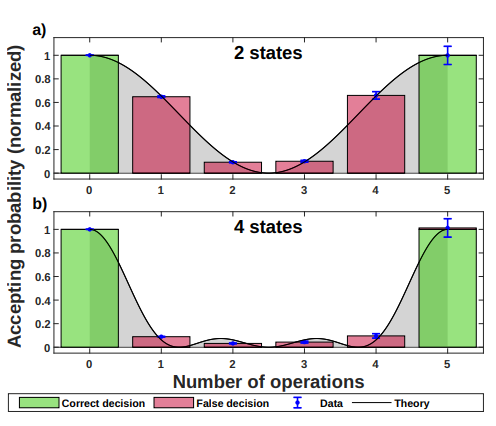
\includegraphics[width=0.3\textwidth]{2states_4states.png}
\end{frame}


\begin{frame}[t]{Recognizing MOD\_11}
  \begin{itemize}
    \item Only 4 states gives good results(as opposed to 5 for classical)
  \end{itemize}
  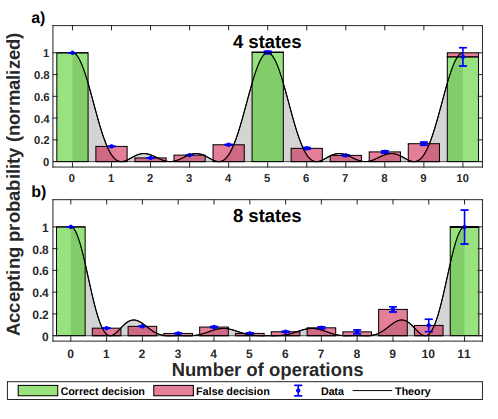
\includegraphics[width=0.3\textwidth]{4states_8states.png}
\end{frame}


\begin{frame}[t]{Summary}
  \begin{itemize}
    \item Photonic realization of QFA
    \item Structured photons as multi-qubit states
    \item Demonstrates efficiency with 2-qubit QFA compared to classical FA (4 instead of 5 staes / 8 instead of 11 states)
  \end{itemize}
\end{frame}


% 
\begin{frame}{Determination of the photon PDF}
  \begin{columns}[T]
    \begin{column}{0.59\textwidth}
      Initially the photon PDF has been determined in different ways:
      \begin{itemize}
        \item physical model: sensitive to underlying model
        \item fitting: data does not provide strong constraints
      \end{itemize}

      \vspace*{0.5em}
      However with the LUXqed approach it can be computed perturbatively \\
      based on the observation that the heavy-lepton production cross-section can be written in two ways:
      \begin{itemize}
        \item in terms of structure functions $F_2$, $F_L$
        \item in terms of PDFs (including the photon)
      \end{itemize}

      \vspace*{0.5em}
      luxQED result {\color{gray}\small[Manohar, Nason, Salam, Zanderighi: 1607.04266, 1708.01256]}:
      \vspace*{-0.8em}
      \begin{equation*}
        \begin{split}
          & x \gamma(x, \mu^2)
          =
          \frac{2}{\alpha (\mu^2)} \int\limits_x^1 \frac{dz}{z}
          \Biggl\{ \int_{m_p^2x^2 \over 1-z}^{\mu^2 \over 1-z} \frac{dQ^2}{Q^2}
          \alpha^2(Q^2) \Biggl[ -z^2 F_L(x/z, Q^2) \\
          & + \left( z P_{\gamma q}(z) + \frac{2 x^2 m_p^2}{Q^2} \right)
          F_2(x/z, Q^2)\Biggr] - \alpha^2(\mu^2) z^2 F_2(x/z, \mu^2)\Biggr\}
        \end{split}
      \end{equation*}
    \end{column}

    \begin{column}{0.39\textwidth}
      \vspace*{-2.5em}
      \begin{figure}
        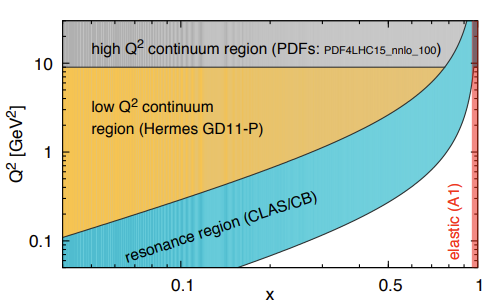
\includegraphics[width=0.89\textwidth]{figures/dataluxqed.png}
        \caption*{Input to construct $F_2$ and $F_L$}
        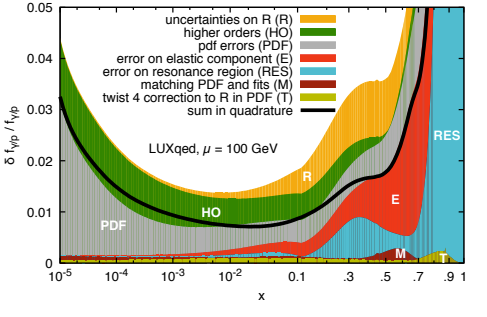
\includegraphics[width=0.89\textwidth]{figures/luxQED_uncs.png}
        \caption*{Sources of uncertainty}
      \end{figure}
    \end{column}
  \end{columns}
\end{frame}


\begin{frame}{LUXqed PDF determinations}
  LUXqed has been used in all of the most recent QED PDFs:
  \begin{itemize}
      \item LUXqed\_plus\_PDF4LHC15 {\color{gray}\small [1607.04266]}
      \item LUXqed17\_plus\_PDF4LHC15 {\color{gray}\small [1708.01256]}
      \item MMHT2015qed {\color{gray}\small [1907.02750]}
      \item NNPDF3.1luxQED {\color{gray}\small [1712.07053]}
      \item CT18lux and CT18qed {\color{gray}\small [2106.10299]}
      \item MSHT20QED {\color{gray}\small [2111.05357]}
      \item MSHT20qed\_an3lo {\color{gray}\small [2312.07665]}
      \item NNPDF4.0QED {\color{gray}\small [2401.08749 ]}
  \end{itemize}
\end{frame}

% \begin{frame}{Results: photon PDF and luminosity}
%   \begin{center}
%     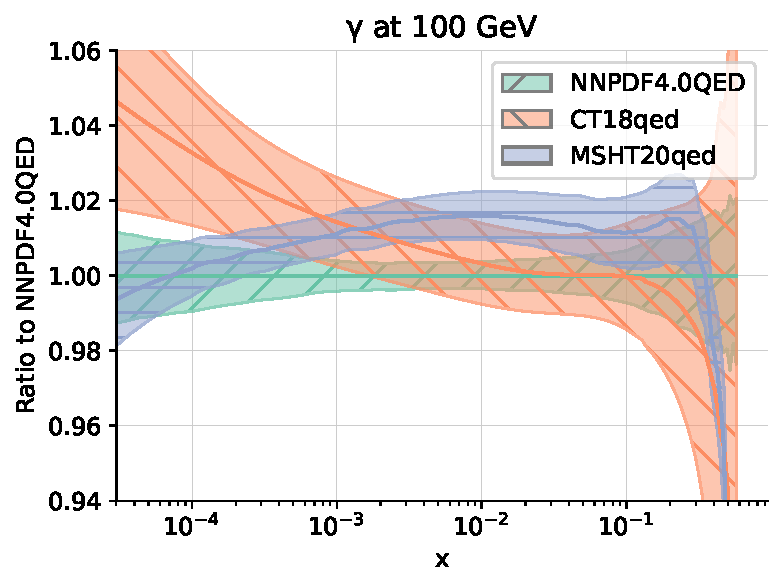
\includegraphics[width=0.3\textwidth]{figures/photon_comparison.pdf}
%     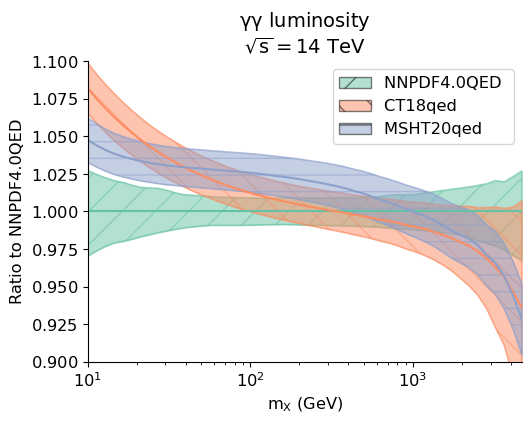
\includegraphics[width=0.3\textwidth]{figures/pp_lumi_comparison.png}
%     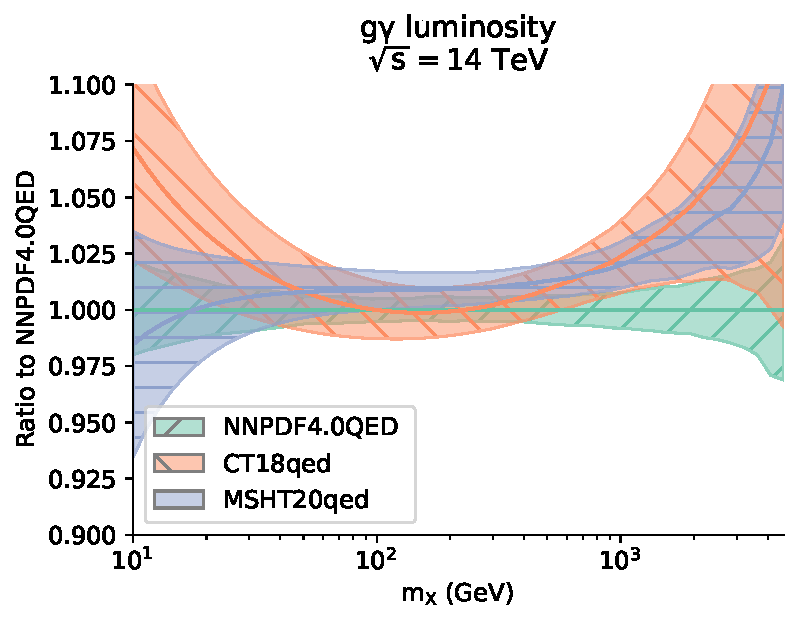
\includegraphics[width=0.3\textwidth]{figures/gp_lumi_comparison.pdf}
%   \end{center}
%   \begin{itemize}
%     \item Because all groups use the luxQED formalism, the photon PDFs agree at percent level
%     \item Luminosity generally in agreement, but differ at very small and very large invariant mass
%   \end{itemize}
% \end{frame}


% ============================================================================


\begin{frame}{Incomplete higher order uncertainties covmat}
  \begin{itemize}
    \item We construct an IHOU matrix following a similar approach by varying the subleading functions
    \item IHOU are independent of MHOU so the uncertainties are added in quadrature
    $$C = C_\mathrm{exp}+C_\mathrm{MHOU}+C_\mathrm{IHOU}$$
  \end{itemize}

  \begin{columns}
    \begin{column}{0.49\textwidth}
      \begin{figure}[!t]
        \centering
        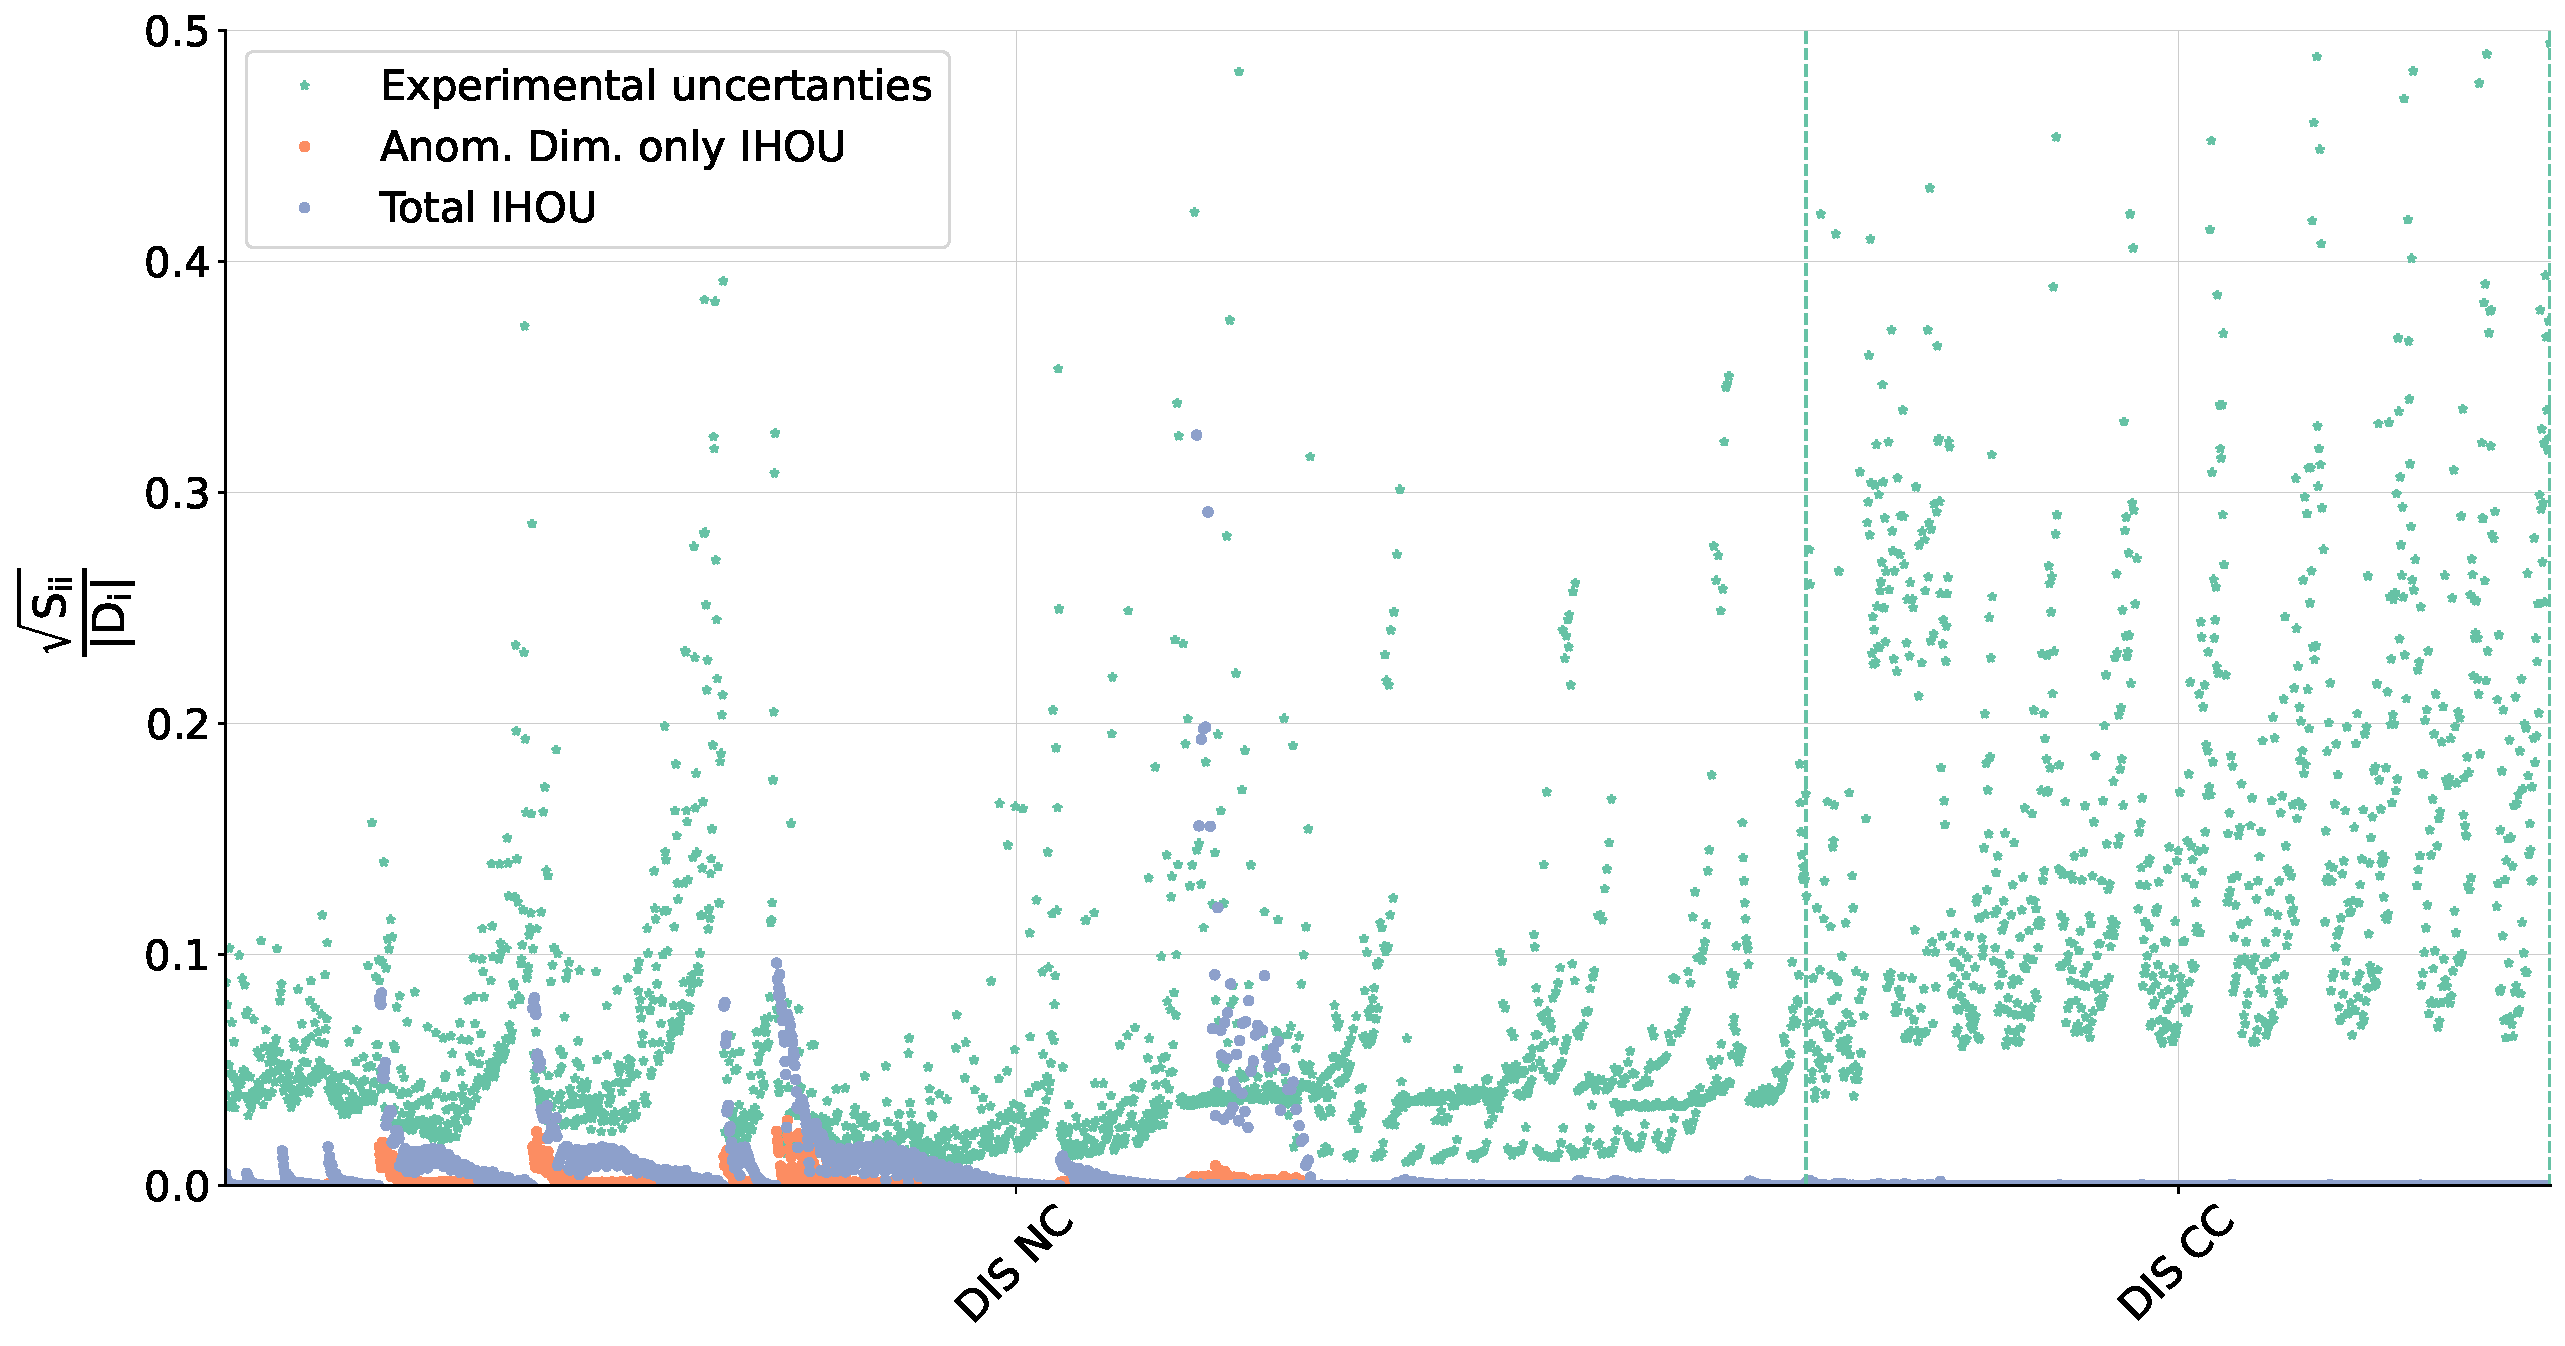
\includegraphics[width=.9\textwidth]{figures/diag_cov_dis_ihou.pdf}
        \caption*{IHOU have a large effect on small-$x$, low-$Q$ DIS data
        }
      \end{figure}
    \end{column}
    \begin{column}{0.49\textwidth}
      \begin{figure}[!t]
        \centering
        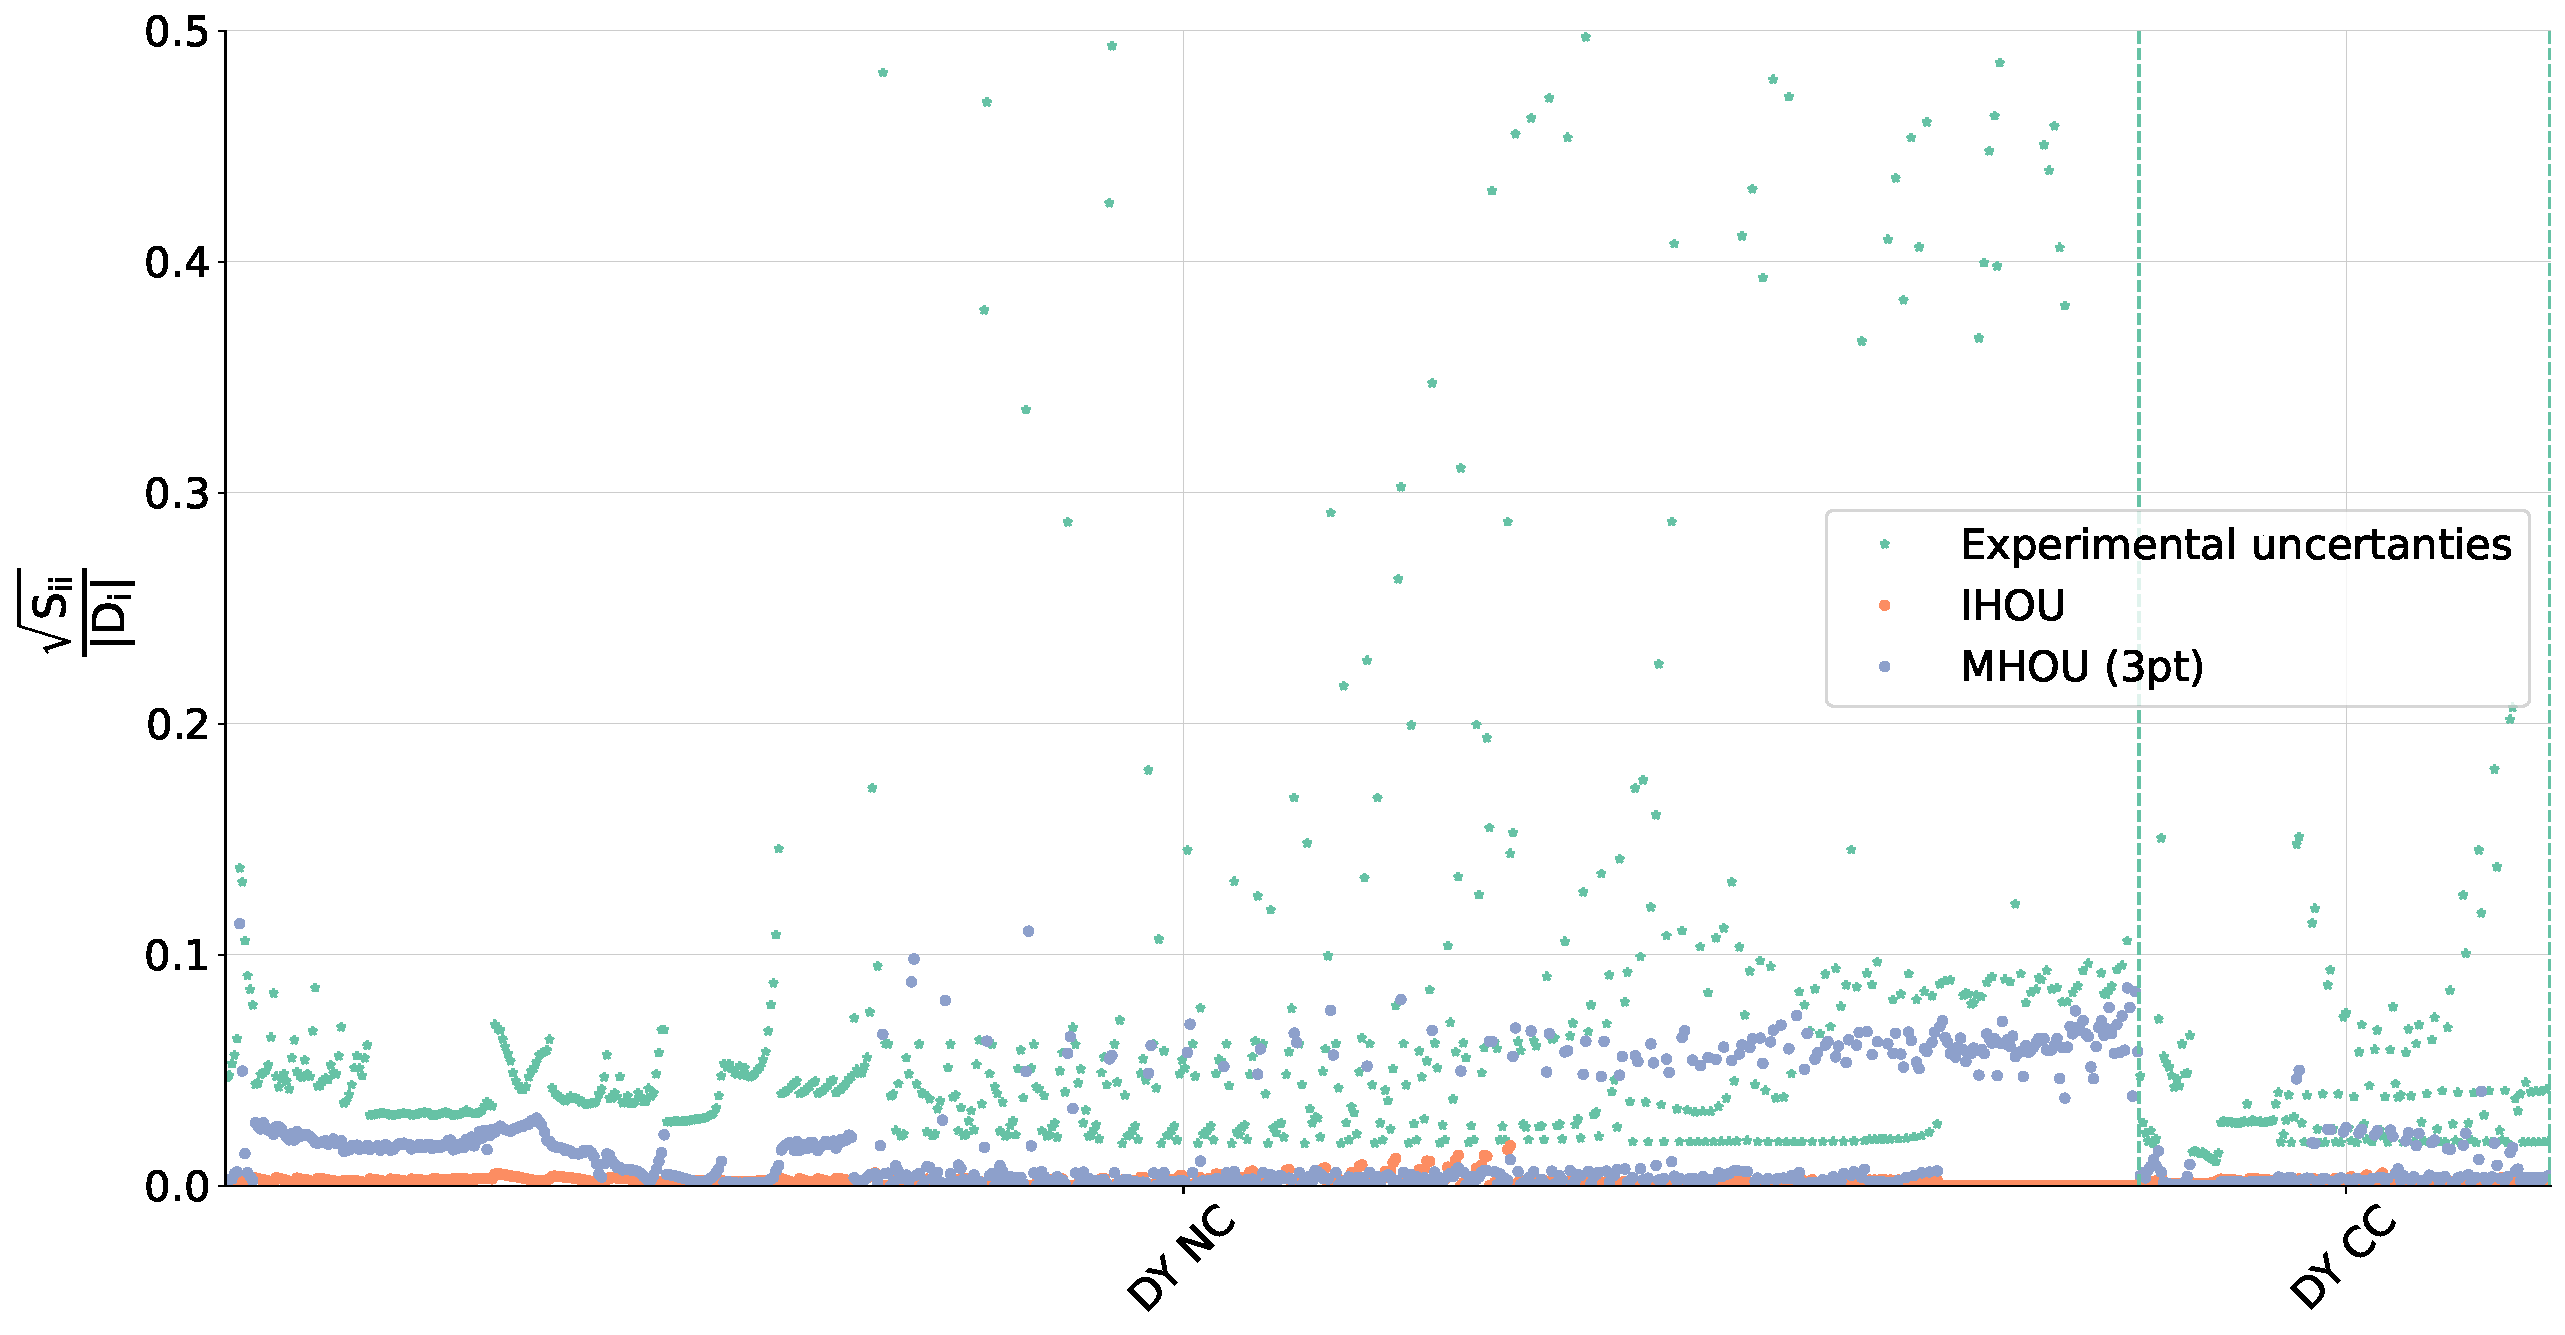
\includegraphics[width=.9\textwidth]{figures/diag_cov_dy_ihou_3pt_mhou.pdf}
        \caption*{NNLO MHOU included where N3LO not available \\
          MHOU can similar magnitude as the experimental uncertainty
        }
      \end{figure}
    \end{column}
  \end{columns}


\end{frame}

% \begin{frame}{Magnitude of theory uncertainties}
% % show that for certain processes th unc is of same size as exp unc.
% \end{frame}

% ============================================================================

\begin{frame}{Impact of MHOUs at N3LO}
  \begin{figure}[!t]
    \centering
    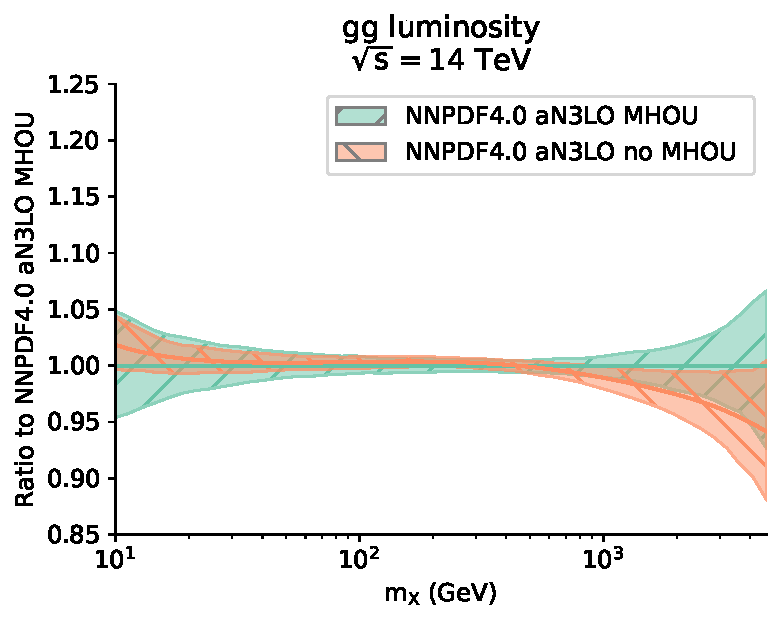
\includegraphics[width=0.45\textwidth]{figures/gg_plot_lumi1d.pdf}
    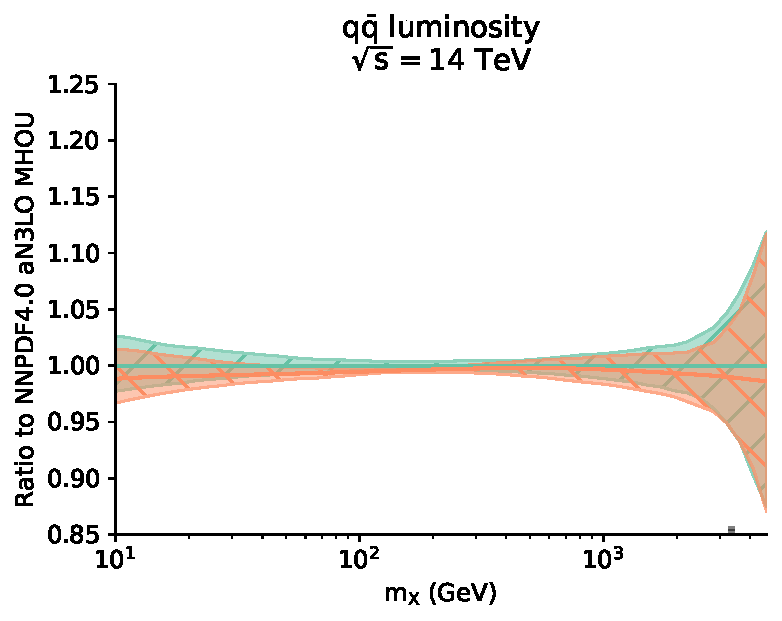
\includegraphics[width=0.45\textwidth]{figures/qqbar_plot_lumi1d.pdf}
  \end{figure}
  \begin{itemize}
    \item Non-negligible impact of MHOUs even at N3LO
    \item[$\Rightarrow$] reason to include exact N3LO calculations for hadronic processes
  \end{itemize}
\end{frame}


% \begin{frame}{Comparison to MSHT20}
%   \begin{figure}[!t]
%     \centering
%     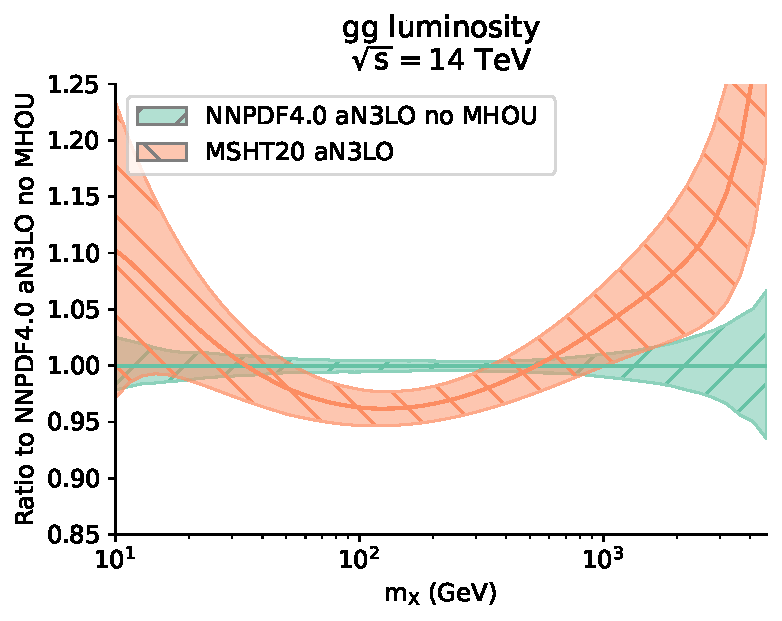
\includegraphics[width=0.45\textwidth]{figures/gg_plot_lumi1d_msht20.pdf}
%     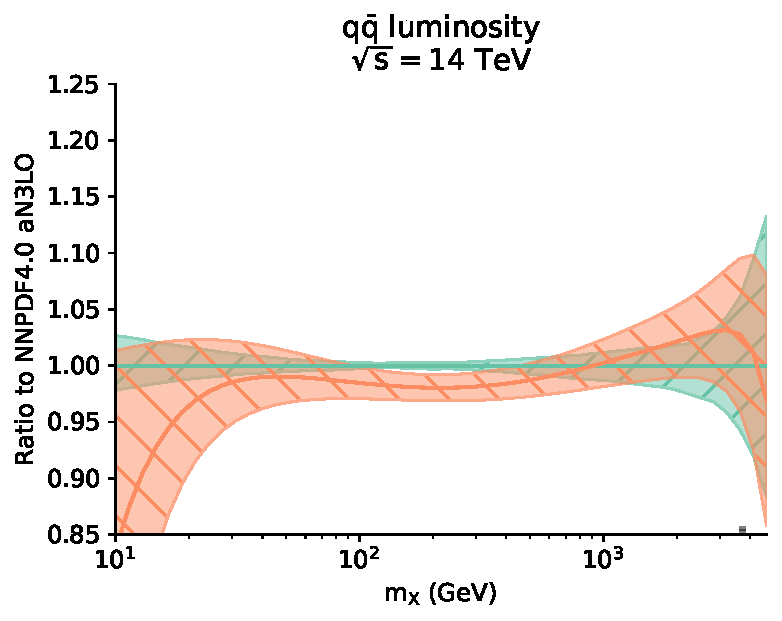
\includegraphics[width=0.45\textwidth]{figures/qqbar_plot_lumi1d_msht20.pdf}
%   \end{figure}
%   \begin{itemize}
%     \item Good agreement with MSHT20 for the quark luminosities
%     \item Also for gluon luminosities, except around the Higgs mass and high-mass
%     \item Similar data but different methodology (including splitting function parametrization)
%   \end{itemize}
% \end{frame}



\end{document}





